%latex model.tex
%bibtex model
%latex model.tex
%latex model.tex
%pdflatex model.tex

%se poate lucra si online (de ex www.overleaf.com)


\documentclass[runningheads,a4paper,11pt]{report}

\usepackage{algorithmic}
\usepackage{algorithm} 
\usepackage{array}
\usepackage{amsmath}
\usepackage{amsfonts}
\usepackage{amssymb}
\usepackage{amsthm}
\usepackage{caption}
\usepackage{comment} 
\usepackage{epsfig} 
\usepackage{fancyhdr}
\usepackage[T1]{fontenc}
\usepackage{geometry} 
\usepackage{graphicx}
\usepackage[colorlinks]{hyperref} 
\usepackage[latin1]{inputenc}
\usepackage{multicol}
\usepackage{multirow} 
\usepackage{rotating}
\usepackage{setspace}
\usepackage{subfigure}
\usepackage{url}
\usepackage{verbatim}
\usepackage{xcolor}

\geometry{a4paper,top=3cm,left=2cm,right=2cm,bottom=3cm}

\pagestyle{fancy}
\fancyhf{}
\fancyhead[LE,RO]{Automated System for Social Density}
\fancyhead[RE,LO]{AlwaysRight}
\fancyfoot[RE,LO]{ITSG 2020-2021}
\fancyfoot[LE,RO]{\thepage}

\renewcommand{\headrulewidth}{2pt}
\renewcommand{\footrulewidth}{1pt}
\renewcommand{\headrule}{\hbox to\headwidth{%
  \color{lime}\leaders\hrule height \headrulewidth\hfill}}
\renewcommand{\footrule}{\hbox to\headwidth{%
  \color{lime}\leaders\hrule height \footrulewidth\hfill}}

\hypersetup{
pdftitle={artTitle},
pdfauthor={name},
pdfkeywords={pdf, latex, tex, ps2pdf, dvipdfm, pdflatex},
bookmarksnumbered,
pdfstartview={FitH},
urlcolor=cyan,
colorlinks=true,
linkcolor=red,
citecolor=green,
}
% \pagestyle{plain}

\setcounter{secnumdepth}{3}
\setcounter{tocdepth}{3}

\linespread{1}

% \pagestyle{myheadings}

\makeindex


\begin{document}

\begin{titlepage}
\sloppy

\begin{center}
BABE\c S BOLYAI UNIVERSITY, CLUJ NAPOCA, ROM\^ ANIA

FACULTY OF MATHEMATICS AND COMPUTER SCIENCE

\vspace{6cm}

\Huge \textbf{Automated System for Social Density}

\vspace{1cm}

\normalsize -- ITSG report --

\end{center}


\vspace{5cm}

\begin{flushright}
\Large{\textbf{Team members}}\\
Berciu Liviu, SE, 258, blis2031@scs.ubbcluj.ro \\
Cotrau Andreea, SE, 258, cais2043@scs.ubbcluj.ro \\
Tamas Florin, ICA, 256, tiic2020@scs.ubbcluj.ro \\
Ungur Maria, ICA, 256, umic2022@scs.ubbcluj.ro \\
\end{flushright}

\vspace{4cm}

\begin{center}
2020-2021
\end{center}

\end{titlepage}

\pagenumbering{gobble}

\begin{abstract}
The outbreak of the Coronavirus disease (COVID-19) has spread extremely quick across the world, and therefore the concept of social distancing and the avoidance of physical contact became a major and efficient measure that can help against the spread of the virus. As people come together in crowds, it is more likely that they will come in contact with someone that has the virus.
Thus, this paper studies the problem of critical density and social distancing, and we propose an application that could help reduce the spread of Coronavirus (COVID-19), by providing a surveillance system which uses YOLOv3, an intelligent algorithm for real-time human detection for institutions, offices and various buildings that would like to monitor if the measures are respected by the people that are present in their spaces and to avoid overcrowding.
Therefore, any building that uses this system will have an overview of the density of people that are present in every room, and this way they could let people that would like to enter a certain area know when the density of that room or space is too high and when the risk of having contact with someone that might be infected increases. This way, a proper density of people can be maintained the whole time and the spread of the virus can be minimized.
We tested the proposed method with subsets from COCO and INRIA datasets, together with real-time snapshots, in order to measure its generality, performance and precision. The experiments showed that the YOLOv3 versions have an acceptable performance for the given task and we presented a comparison between different versions, in order to reach to the conclusion that trade-off between accuracy and performance is an important aspect for real-time computer vision tasks.
\end{abstract}


\tableofcontents

\newpage

\listoftables
\listoffigures
\listofalgorithms

\newpage

\setstretch{1.5}


\newpage

\pagenumbering{arabic}

\chapter{Introduction}
\label{chapter:introduction}

\section{What? Why? How?}
\label{section:what}

The year 2020 has proven to be different from many points of view, the main reason being the Covid19 pandemic that took by surprise the entire globe. People had to adapt to this peculiar virus and adopted a set of rules to fight the "invisible enemy". Among those, we find the so-called "social distancing" which basically can be translated as a safe distance maintained between two persons. This rule was supported by the World Health Organization so it quickly gained popularity among the countries. It became a standard and a thing that had to be considered in our day to day life.
\begin{itemize}
	\item \textbf{What is the (scientific) problem?} - The ordinary life we live has to address the social distancing problem now in all indoor spaces (classrooms, offices, buses, supermarkets and others). This has a huge impact on the overall society's well being. Nonetheless, this has to be monitored and maintained. To do such a thing, companies have adapted: employed people just for surveillance, to insure the distance is kept or adjusted the employment contract for some in order to add a chore to their daily list of actions. In most of the cases, this can be automated. We identified the scientific problem as to automatically identify the number of people in a space, as well as the distance between people. Moreover, provide this information in a nice manner, in a web application to the person interested, be it a manager of a space, the bus driver or the class teacher. It should be structured as a dashboard where all the details are displayed.
	\item \textbf{Why is it important?} - Finding an automated solution for this problem would mean saving a lot of time and effort from the employees in charge. It is also an actual, real problem that the society is facing, a problem of momentum. We consider that it is a perfect situation in which machine learning can improve the quality of life, maybe even help save it. 
	\item \textbf{What is your basic approach?} - Our team is developing a system of image recognition, specifically, person recognition from images taken from web cameras or surveillance cameras. We will use some trained models to identify the person's contour in the image and count the number of persons in a room. The next step would be to translate the image in three dimension and check the distance between the persons. The final output will be displayed in a dashboard via a web application.
\end{itemize}

Related work in the area is found on person recognition, and on 3D image processing, but our main contribution would be addressing a real problem of social distancing and creating the application.
% A short discussion of how it fits into related work in the area is also desirable. Summarize the basic results and conclusions that you will present. 


\section{Paper structure and original contribution(s)}
\label{section:structure}

The research presented in this paper advances the theory, design, and implementation of several particular models. 

The main contribution of this report is to present an intelligent algorithm for solving the problem of critical density and social distancing.

The second contribution of this report consists of building an intuitive, easy-to-use and user friendly software application. Our aim is to build an algorithm that will help reduce the spread of Coronavirus (COVID-19), by providing a surveillance system which uses real-time human detection for institutions, offices and various buildings that would like to monitor if the measures are respected by the people that are present in their spaces and to check when the density of certain areas reach a critical point, in order to avoid overcrowding, and to ensure a safer place with less human contacts.

The third contribution of this thesis consists of providing a comparison between the state of art and our approach.


The present work contains eight bibliographical references and is structured in five chapters as follows. The first chapter is a short introduction in our study and what it is about and why it is important and our reasons that were behind choosing this topic. The second section describes the scientific problem and considers the advantages and disadvantages of our approach. The third chapter describes the state of art and how our method is different. The fourth chapter provides the investigated approach, together with the tools and technologies that were used in order to implement it. The fifth chapter presents the chosen methodology, and a comparison between the results obtained from different datasets. At the same time, also the social impact of the application is presented in this section. The final chapter presents our conclusion and final results, and the future work that could be done in order to improve our system.



\chapter{Scientific Problem}
\label{section:scientificProblem}


\section{Problem definition}
\label{section:problemDefinition}


Nowadays we have a rather unusual situation, because of the COVID-19 pandemic. There are restrictions everywhere we go, especially inside. And these restrictions are meant to protect the people and hinder the spread of the Corona virus. And the most problematic spaces are represented by the public spaces that are inside, where the virus can be easily spread to the all the persons that will be present in that room during a period of time. Even though it was recommended to practice social distancing , there are many cases where from various reasons this is not respected.

Therefore, the goal of our system is to diminish the spread of Corona virus and to protect people from getting infected and spreading it further more to their close relatives and friends. At the same time, we plan on helping all the public and private buildings that would like to keep every person that is present in different rooms inside their building safe, by tracking every person inside a room, together with the information regarding the social distancing.

Our system is provided as a web page, where the user is provided with a live feed for every room and real time pictures that represent the status of a room at a certain time,  accompanied by statistics, such as the number of people and if the room exceeds the allowed number of people or not.

Thus, the above mentioned problem can be solved by our system, that provides an intelligent algorithm for person recognition, in order to identify the people that are present within a certain room.
The web page was designed to communicate with a machine learning server via REST services, and it outputs the received prediction. In order for the machine learning server to receive an image, it communicates with a raspberry PI server that captures the image upon request.

As benefits and advantages of using our system, the most important one is the fact that people can be more safe and the spread of Corona virus can be diminished. At the same time, the personnel of different institutions, companies and any private or public building, can also keep the distance from the clients or just the people inside the room, and they wouldn't have to personally check if the people respect the restrictions regarding the number of persons that are inside a room or if they respect the distance between them or not.
They can just use our system and track all the people from any room, while keeping also the distance from them. They can see the people that are inside a room and they can get real time information regarding the status of any room. When the number of persons allowed in a certain room is exceeded, an alert will start and the responsible people can easily see from which room it comes from, and this way they can take action.

One disadvantage that we were able to identify, is the fact that the people who would like to use our system, will need to buy cameras and install them in all the rooms where they would like to track the people. This is needed in order to provide our system with real time data, such that it shows the live status of a certain room, and also various snapshots, taken at a certain desired moment.

\section{Input}
\label{section:input}

The input for our system is represented by the camera(or more cameras) that records a room and transmits the information of a certain room live.

\section{Output}
\label{section:output}

The output can be represented by a processed image that was taken by the camera at a specific moment. At the same time, the output can be also a live processed recording from a room.
Any of these output types will recognize the number of people within a room and will trigger an alert when the allowed number of people is exceeded.

\chapter{State of the art/Related work}
\label{chapter:stateOfArt}


In this chapter we present a few methods that were used in order to monitor the social distancing between people for COVID-19.

Firstly, we will take a look at \cite{OpenCV}, where social distancing is tracked in public places.

\begin{itemize}
	\item \textbf{What is their problem and method?} - In this surveyed paper, they are trying to keep track of the social distancing between people in public places, by creating a social distancing detector. They consider that social distancing is present when the physical distance is at least 1 meter (3 feet) between a given pair of people. Therefore, they created a surveillance method that uses Open-CV, Computer vision and Deep learning. This way, overcrowding can be avoided and the persons are tracked, by the cameras from closed circuit television (CCTV) and Drones. People are detected through the mentioned cameras, by using object detection, and the distance between them is computed. This is implemented by computing the Euclidean distance between a pair of two people, which is at first calculated in pixels and then it is compared with the standard distance of 1 meter. If it is less then the standard distance, then the local police authorities will get notified.
	\item \textbf{How is our problem and method different?} - Our problem is a little bit different than the one from the mentioned paper, because we try to monitor social distancing between people that are present in certain rooms or certain areas that belong to a particular building or institution, and not outside on the public streets. At the same time, we are using surveillance cameras in order to track the people, while they are using closed circuit television (CCTV) and Drones. The implementation is also done differently, since we are using  YOLO for object detection, while their implementation was done by training a cascade classifier for head detection from the scene, by using Haar features through OpenCV.
	\item \textbf{Why is our problem and method better?} - Our problem takes into consideration the needs of the institutions, schools and various buildings that are trying to maintain social distancing between people. Therefore, we come to their help and we try to make their lives easier, by providing a solution that will let them know when social distancing is not respected inside their building. At the same time, we use YOLO  (You Only Look Once) for real time object detection, which is considered to have less shortcomings and to be much faster, when it comes to providing accurate results.
\end{itemize}


Next, we will take a look at \cite{CriticalDensity}, where social distancing is monitored together with the critical density in different places.

\begin{itemize}
	\item \textbf{What is their problem and method?} - In this paper, they try to monitor the distance between people through an active surveillance system, and to slow down the spread of the disease by warning them, since individuals are not used to tracking the requires distance, which is considered to be of 2 meters (6 feet). At the same time, since inflow can decrease the occurrence of social distancing violations, they are also trying to measure the social density in a region of interest (ROI). But, people's rights are breached when they are labeled and recorded for not following the required measures in free-societies. Therefore, they propose a solution based on real-time social distancing detection and warning system, that consider some ethical factors, like the following: the system never records/caches data and the warnings don't target the individuals. They use a monocular camera and deep learning based object detectors, that measure the social distancing. When a violation is detected, a warning signal is emitted to warn the whole crowd, without targeting the specific individual that breached the required measure. At the same time, when the social density is higher than the critical value, a signal will be sent from the system, such that the inflow is modulated into that region of interest. This is done by advising people to not enter into that region of interest when the density is over that critical value.
	\item \textbf{How is our problem and method different?} - Our problem is slightly different than the one from the surveyed paper, since we try to monitor social distancing between people that are present in certain rooms or certain areas that belong to a particular building or institution, while they are tracking individuals that are present in various free-societies. At the same time, they mention using real-time camera system, specifically a monocular camera. The implementation is also done differently, since we are using  YOLO for object detection, while they detect pedestrians with a deep CNN model, that was trained on a real-world dataset, like the Oxford Town Center dataset and the NYC Train Station dataset. But they mention that in the future they plan on using YOLO v4 for the detection, in order to have a better performance and speed of the detection.
	\item \textbf{Why is our problem and method better?} - Our problem tries to come to the help of any institution or company during this times, in order to provide a way of maintaining the social distancing and the given regulations. Our solution will let the owners know when the conditions are not respected and when the density is higher in certain areas than the allowed number, such that they can take care of the safety of everyone that comes into their building. While their plan for the future is to use YOLO v4 for the detection, we already use it and we can say that we managed to acquire a much faster program, with a better performance in retrieving the results.
\end{itemize}


\chapter{Investigated approach}
\label{chapter:proposedApproach}

\section{Algorithm description}
\label{section:solution}
Our algorithm is composed of three main steps: capturing the image from a room, person detection and distance approximation between pairs of person bounding boxes.

\begin{figure}[H]
	\centerline{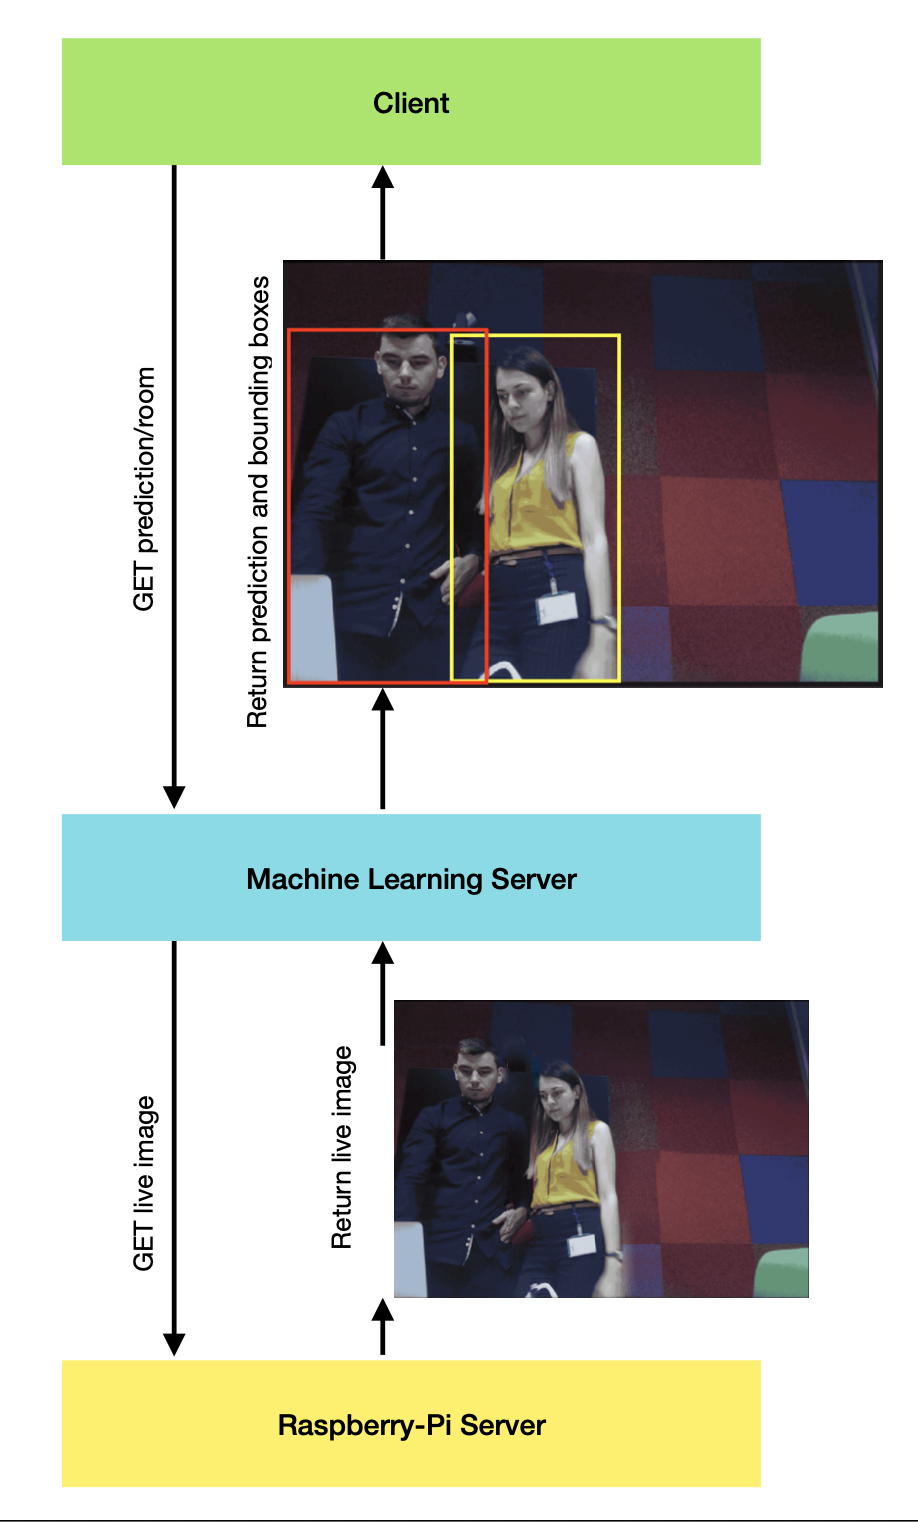
\includegraphics[scale=0.45]{Flow-diagram.png}}  
	\caption{The investigated approach basic flow.}
	\label{Flow-diagram}
\end{figure}

\subsection{Person Detection}
For the person detection algorithm, we have chosen to use a state of the art machine learning approach, namely the third version of YOLO \cite{YOLO}. This choice was mainly done because the YOLO algorithm presents the best trade-off between accuracy and performance which is an important aspect for analyzing the real-time computer vision tasks. The YOLO model has several advantages over classifier-based systems. The novel approach that the model brings is that it looks at the whole image at test time so its predictions are informed by global context in the image. It also makes predictions with a single network evaluation unlike systems like R-CNN which require thousands for a single image, proving that the model is more than 1000x faster than R-CNN and 100x faster than Fast R-CNN. After some bench testing, we selected YOLOv3-tiny for our algorithm. Once the bounding boxes are detected by the model, the next step in our algorithm is computing the distance between persons in order to provide information on the social distancing status. 
\algsetup{indent=1em, linenosize=\footnotesize}
\begin{algorithm}
	\caption{Predict bounding boxes}
	\label{NGalg}
		\begin{algorithmic}
		\STATE \textbf{BEGIN}
  		\STATE @ Predict bounding boxes for the persons in the image
  		\STATE @ Input param: image \\
  		\STATE @ Convert the PIL image to a CV image \\
  		\STATE cv\_image $\leftarrow$ pil2opencv(image) \\
  		\STATE img\_darknet $\leftarrow$ pydarknet.Image(cv\_image) \\
  		\STATE detections $\leftarrow$ model.detect(img\_darknet) \\
  		\STATE bounding\_boxes $\leftarrow$ getBoundingBoxedFromDetections(detections) \\
  		\STATE \textbf{END}
\end{algorithmic}
\end{algorithm}

\subsection{Room monitoring system}
For monitoring the room, the system consists of a Raspberry-Pi board and an auxiliary camera(Raspberry-Pi Camera v2). The Raspberry-Pi device exposes a REST API that can be used to retrieve live images from the camera. The camera is controller by using the Android Things API and takes a snapshot of the room whenever the client sends a GET request to the endpoint.

\begin{figure}[H]
	\centerline{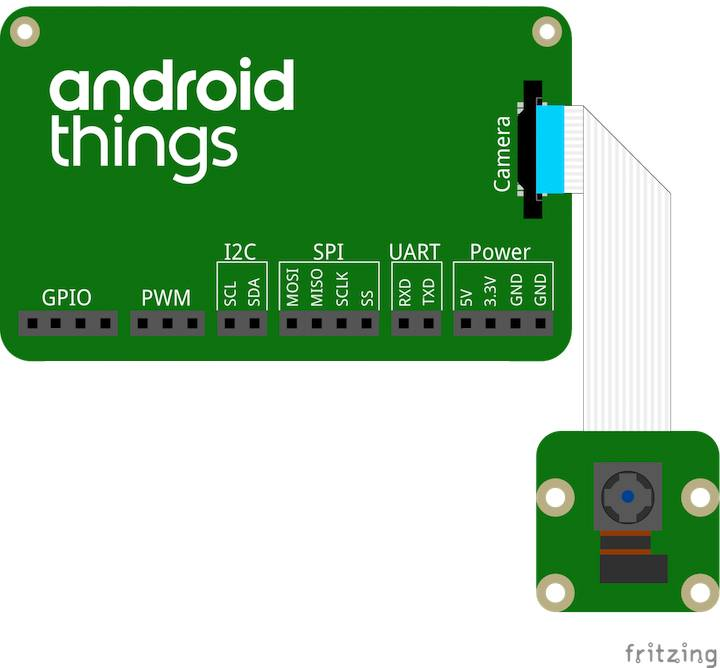
\includegraphics[scale=0.3]{schematics.jpg}}  
	\caption{The schema of the hardware system.}
	\label{Hardware schema}
\end{figure}

\section{Tools and technologies}

\label{section:tools}

Our approach is composed of four big component parts (C) and the two process parts (P):
\begin{itemize}
    \item \textbf{Machine Learning Server (C)} - uses YOLOv3 for person recognition. Python is used in order to develop this server, together with Flask framework, that helps with building APIs in Python. The editor that we used is PyCharm, and it already has an integrated debugger, making it easier to find and fix errors.
    \item \textbf{PI Server (C)} - implemented using Java as a programming language, which was chosen because of Android Things API that is used in order to access the Raspberry-Pi Camera. We used IntelliJ IDEA as the main environment of implementation, providing us with the correct tools for debugging, error detection and helpful features for our programming language. Unit tests are an alternative when it comes to testing our server.
    \item \textbf{User Interface (C)} - created using React JS, namely a Javascript framework used for developing web applications. Visual Studio Code was used as a development environment, because of its built-in support for coding and the ease of debugging that it provides. Different libraries are used to ensure a wonderful user experience and an unyielding connection to the machine learning server. For testing, we used Component unit testing specific to React. Also, a VS Code debugging tool was used, ensuring stability when deploying our app.
    \item \textbf{Hardware system (C)} - a Raspberry-Pi device together with the Raspberry-Pi Camera v2. In order to develop code for the device, we run Android Studio, which allows us to do deploying of the solution and debugging.
    \item \textbf{CI - Continuous Integration (P)} - for the continuous integration we use Github Actions for building the components. We now have one action for each system component. It handles the dependencies and the integration and is run after each commit.
    \item \textbf{CD - Continuous Deployment (P)} - tightly coupled with the point above, we have the continuous deployment process which is accomplished through Github Actions and Heroku PaaS. We host on Heroku the web application as well as the Machine Learning Server. After a successful build, another Github Action deploys the application components.
\end{itemize}

\section{Testing}
\label{section:testing}

An important part of every software, testing is a must for a system that prizes itself in it's ability to detect people inside different types of spaces. We have approached this part of our project development in two ways: \textbf{manual testing} for the Python server and \textbf{React Testing Library} for the Web client.

\subsection{Manual testing}

We have chosen to manually test the YOLO server since it provides a lot flexibility throughout the QA process. It allows us to find model errors and bugs using our AI experience and critical thinking. While doing manual testing, we interacted directly with the system and ensured that it is was working as required. 
In Figure 4.3, we have an example on how we proceeded with our method. We provided different people images to the algorithm and expected an output where every person has a coloured border surrounding their body. So far, nothing went wrong.

\begin{figure}[H]
	\centerline{\includegraphics[scale=0.45]{testing_diagram.jpg}}  
	\caption{Manual testing flow.}
	\label{Flow-diagram}
\end{figure}

\subsection{React Test Framework}
Our Web UI component is implemented in React JS. Delivering a professional looking webpage is not scalable if, with every new release, we don't have a proper testing plan to make sure everything works as expected and nothing changed for the worst. Delivering good results for our clients is our top priority, hence, for both efficiency and a better code understanding, we have chosen to use the default \textbf{React Testing Library}.

The React Testing Library is a very light-weight solution for testing React components, providing light utility functions on top of \textbf{react-dom} and \textbf{react-dom/test-utils}. This way, better software practices are encouraged. Its primary guiding principle is \textit{The more your tests resemble the way your software is used, the more confidence they can give you}.


 We have added unit-tests for the following pages:
 \begin{itemize}
     \item Home
     \item About Us
     \item Statistics
 \end{itemize}
 
 Our test mainly include checking if the elements are rendered and if required information, such as the presentation video, team members and other details are shown to the user.

\chapter{Application (numerical validation)}
\label{chapter:application}

Since our approach is based on the pre-trained version of the YOLO model, we performed our experiments having in mind two aspects: time for processing and accuracy. The reason behind this was to balance these two. The experiments consisted in choosing all of the available weights for the pre-trained models and modifying the size of the images that they work on.

\section{Methodology}
\label{section:methodology}
In this section we will describe the methodology used for testing the model.

One of the methodologies was the usage of different network weights: the weights for the full model and the weights for the modified model(which contains a lower number of convolutional layers - known as YOLOv3-tiny).

Another methodology was the usage of different sizes for the input image: 320x320, 416x416 and 608x608. We wanted to measure the link between the image size and the precision of the network.

% \begin{itemize}
% 	\item What are criteria you are using to evaluate your method? 
% 	\item What specific hypotheses does your experiment test? Describe the experimental methodology that you used. 
% 	\item What are the dependent and independent variables? 
% 	\item What is the training/test data that was used, and why is it realistic or interesting? Exactly what performance data did you collect and how are you presenting and analyzing it? Comparisons to competing methods that address the same problem are particularly useful.
% \end{itemize}

\section{Data}
\label{section:data}

For the dataset, we selected some subsets from the COCO an INRIA datasets. We will dive in details below.

\subsection{COCO dataset}
A largely available dataset is COCO \cite{COCODataset} - Common Objects in Context and was used to train the YOLOv3 model. The COCO dataset contains 80 classes of objects from which we mainly chose the \textit{"person"} label. The results of training the model on this dataset can be seen in table \ref{tab3COCO}

\subsection{INRIA dataset}
Our main experiment dataset was INRIA \cite{INRIADataset} - a dataset which contains images from several different sources such as: the GRAZ01 dataset, images from personal image collections and a few images taken from the web using Google images. The dataset only contains images of upright persons, each person having a height greater than 100cm. A particular issue with this dataset is represented by the fact that some annotations may not be right, for example, some portions of annotated bounding boxes may be outside or inside the object.

\section{Results}
\label{section:results}

Our initial intuition was to take a look at the original benchmark of the author of YOLO algorithm which was completed on the COCO dataset and was run on a Pascal Titan X. The YOLO algorithm itself has multiple versions that are suited for specific usecases. We compared the 5 algorithms as seen below. As we can observe, the YOLOv3-320 version of the algorithm is the best in terms of performance with the drawback that we lose precision. This is a trade-off that we accepted due to the fact that we want to extend the system into a real-time scenario.

For the metrics used in comparison, we focused on mAP (mean Average precision) which is a popular metric in measuring the accuracy of object detectors like Faster R-CNN, SSD, etc. Average precision computes the average precision value for recall value over 0 to 1. Also, we chose FPS (Frames Per Second) as an indicator of the real-time applicability of the algorithm.

\begin{table}[htbp]
	\caption{YOLOv3 algorithm benchmark on COCO dataset}
	\label{tab3COCO}
		\begin{center}
			\begin{tabular}{p{100pt}c c c c}

				\textbf{Model}& \textbf{Dataset}& \textbf{mAP}& \textbf{FPS} \\
				\hline\hline
 				YOLOv3-320& COCO& 51.5& 45 \\
 				YOLOv3-416& COCO& 55.3& 35 \\
 				YOLOv3-608& COCO& 57.9& 20 \\
 				YOLOv3-tiny& COCO& 33.1& 220 \\
 				YOLOv3-spp& COCO& 60.6& 20 \\
			\end{tabular}
		\end{center}
\end{table}


In order to further investigate the time constraints of each algorithm, we performed some additional tests on a subset of the INRIA dataset, where we focused of the time that it takes the algorithm to parse an image. The process consisted in running the algorithm on a set of 60 images. In this way, we are aiming to get a better overview on the applicability of YOLOv3 on the task of person detection. The experiment was run on an Intel Core i5 Quad Core, with a frequency of 2.3GHz, demonstrating that for a better performance in terms of precision, we would need a better GPU. 

\begin{table}[htbp]
	\caption{YOLOv3 algorithm benchmark on INRIA dataset}
	\label{tab3INRIA}
		\begin{center}
			\begin{tabular}{p{100pt}c c c c c}

				\textbf{Model}& \textbf{Dataset}& \textbf{Avg. time(s)}& \textbf{Total time(s)} \\
				\hline\hline
 				YOLOv3-320& INRIA& 4.35& 261.077\\
 				YOLOv3-416& INRIA& 8.24& 494.674\\
 				YOLOv3-608& INRIA& 19& 1140\\
 				YOLOv3-tiny& INRIA& 0.70& 42.291\\
 				YOLOv3-spp& INRIA& 19.2& 1152\\
			\end{tabular}
		\end{center}
\end{table}

An interesting topic which would enhance the performance and bring value to our system would be to compute the distance between two bounding boxes. For the purpose of this paper, we could make this calculating the 2D distance if the camera is somewhere high, like a bird-eye-view, computed to the 2D distance between bounding boxes. However, since the specifications of our camera are limited and the placement of the camera is relatively low, this computations turned out to be not so exact so we decided not to insist on the results, as they don't bring any value for the research. Moreover, other approaches need to be considered for this to work. We will keep this functionality for later stages of the product.

\section{Analysis of Aspects Concerning the Social Impact}
\label{section:social}

Lately, the outbreak of the Coronavirus disease (COVID-19) has spread extremely quick across the world, and therefore the concept of social distancing and the avoidance of physical contact became a major and efficient measure that can help against the spread of the virus. As people come together in crowds, it is more likely that they will come in contact with someone that has COVID-19. While people are not used to paying attention to these measures and cannot always realise that they are in an area with a high risk, where the measures are not properly taken into consideration, they might need some help in knowing when they can enter a certain area. At the same time, even if other people try to keep an eye on a specific place and monitor it in order to maintain the needed measures, it might not always be the best solution.

Therefore, considering these aspects, our application aims at trying to help everyone to fight this battle, by making available a surveillance system that can detect persons with the help of object recognition, in order to keep track of the density of people in different rooms and spaces. If the density inside a certain place is already too high, people will be advised not to enter that place until it is safer for them. Thus, chances of people getting infected decrease, since measuring the density in a certain area and modulating its inflow, can lead to a decrease in the violation occurrences regarding the social distancing. This would benefit the most to the people that have to go in certain places, but it would also benefit the people that are hired in certain institution and that have a job where interaction with customers is needed. This way, all individuals will have a safer environment to go to when it is needed.

At the same time, we try to think also from an ethical point of view, and to consider the individual's rights. And since recording individual's data and labeling those who do not follow the required measures and that do not consider the warnings that concern a higher density in specific places, represents a breach concerning the peoples' rights in public places, we designed a solution that is composed of an artificial intelligence real-time person detection, having a warning system that takes into consideration some ethical factors, like the fact that our application will not record individuals' data, and they will not be targeted directly, since they will only know about the state of the density of people in a place that they are about to enter. Therefore, the people will only get a non-intrusive warning or advice when the density of people is too high, in order to be able to modulate and keep the density under control, without them being directly targeted when they breach any measures.
At the same time, we tested our method across different datasets, in order to be able to measure the performance and generality of our solution, and to provide the needed improvements where they were needed.

\subsection{Improvements to initial approach}
We can discuss about improvements on two directions: one for the machine learning server and one to the client web application.
\begin{itemize}
    \item \textbf{Machine Learning Server} - after an initial functional version of the application, we monitored the performance of the system and we realized that even though we used the fastest version of YOLOv3, the YOLOv3 tiny, there was a high latency between request(i.e. when the user clicks the button "Update" on the dashboard pannel) and response(i.e. when the number of persons is recalculated). So we came with the improvement to implement a worker queue which gets snapshots once every 3 seconds, performs the person recognition task on them and then caches the result for a future request. In this way, the latency reduced significantly. 
    \item \textbf{Client Web Application} - we changed the design after some iterations and included more room monitoring systems. On top of that, we implemented a "Statistics" panel for a better overview of the people-density.
\end{itemize}


\chapter{Conclusion and future work}
\label{chapter:concl}

As a closing word, we can conclude that our system for person-density monitoring in rooms, office buildings or other spaces represents a real benefit in today's coronavirus pandemic, where social distancing is really important. 

The use of YOLOv3 - both tiny and the more powerful version - can be seen as a strength, being easy to integrate and maintain in a system like this, whilst performing good the given task. As seen during this paper, we performed more experiments in order to choose YOLOv3-320 as our final approach. We considered the trade-off between accuracy and performance which is an important aspect for real-time computer vision tasks. 

Another benefit of our system is providing a dashboard web application, offering the user an overview of more spaces/rooms. The statistics panel also provides a better understanding of the density evolution.

As future improvements we would like to include a depth computation in order to enhance the system performance. This will allow the office manager to monitor better the social distancing from each room. With the current setup, this was harder to accomplish as the system would need information about the webcams that it uses as well as their positioning. The Raspberry Pi Cam doesn't have the performance and characteristics for such a task.

Another enhancements that will increase the performance of our current system is the usage of a worker queue. The worker queue retrieves the images from the Raspberry Pi Server and runs the model prediction on them. As a result, the predictions are cached and returned whenever the client accesses the REST API. This offers a smooth experience for the user. This improvement leads to another one, which is the usage of the heavier version of YOLOv3, which has an even better performance. 

We consider that this paper would offer support and encouragement for future endeavors in the social distancing monitoring.


\bibliographystyle{plain}
\begin{thebibliography}{1}
    \bibitem{MonitoringCOVID19}
    Punn, Narinder Singh, Sanjay Kumar Sonbhadra, and Sonali Agarwal. "Monitoring COVID-19 social distancing with person detection and tracking via fine-tuned YOLO v3 and Deepsort techniques." arXiv preprint arXiv:2005.01385 (2020).
    
    \bibitem{TechnologiesForSocialNetworking} Nguyen, Cong T., et al. "A comprehensive survey of enabling and emerging technologies for social distancing Part II: Emerging technologies and open issues." IEEE Access 8 (2020): 154209-154236.
    
    \bibitem{DeepSocial}
    Rezaei, Mahdi, and Mohsen Azarmi. "DeepSOCIAL: Social Distancing Monitoring and Infection Risk Assessment in COVID-19 Pandemic." arXiv preprint arXiv:2008.11672 (2020).
    
    \bibitem{CriticalDensity} Yang, Dongfang, et al. "A vision-based social distancing and critical density detection system for COVID-19." Image video Process. DOI (2020).
    
    \bibitem{LargeScaleComputerVision} Ghodgaonkar, Isha, et al. "Analyzing Worldwide Social Distancing through Large-Scale Computer Vision." arXiv preprint arXiv:2008.12363 (2020).

    \bibitem{OpenCV} Visal, Rucha, Atharva Theurkar, and Bhairavi Shukla. "Monitoring Social Distancing for Covid-19 Using OpenCV and Deep Learning." (2008).
    
    \bibitem{COCODataset} https://cocodataset.org/\#home
    
    \bibitem{INRIADataset} http://pascal.inrialpes.fr/data/human/
    
    \bibitem{YOLO} https://pjreddie.com/darknet/yolo/
    
\end{thebibliography}

\end{document}
